\documentclass[conference]{IEEEtran}
\IEEEoverridecommandlockouts

% Packages essentiels
\usepackage{cite}
\usepackage{amsmath,amssymb,amsfonts}
\usepackage[ruled,vlined,linesnumbered]{algorithm2e}
\usepackage{graphicx}
\usepackage{textcomp}
\usepackage{xcolor}
\usepackage{tikz}
\usetikzlibrary{arrows.meta,positioning}
\usepackage{sansmath}
\usepackage{booktabs}
\usepackage{multirow}
\usepackage{hyperref}
\usepackage{subfig}
\usepackage{comment}
\usepackage{float}
% Package pour numéroter les lignes (à retirer avant soumission finale)
\usepackage{lineno}
\linenumbers

\setlength\linenumbersep{1mm}  % Augmente l'espace entre les numéros et le texte
\renewcommand\linenumberfont{\normalfont\tiny\sffamily\color{gray}}  % Rend les numéros plus discrets

\def\BibTeX{{\rm B\kern-.05em{\sc i\kern-.025em b}\kern-.08em
    T\kern-.1667em\lower.7ex\hbox{E}\kern-.125emX}}




\def\BibTeX{{\rm B\kern-.05em{\sc i\kern-.025em b}\kern-.08em
    T\kern-.1667em\lower.7ex\hbox{E}\kern-.125emX}}

\begin{document}

%\title{MCTN: Réseau d'Attention Multi-Têtes pour le Démosaïquage d'Images Hyperspectrales à partir de Données MSFA}
\title{MCAN-MTD: Descripteur Transformeur Mosaïque pour le Démosaïquage Hyperspectral à partir de MSFA 4$\times$4 sur Images Multispectrales}


\author{\IEEEauthorblockN{LAWSON Latevi Sena}
\IEEEauthorblockA{\textit{Technologie de l'information et de la communication} \\
\textit{IMSP(Institut de Mathématiques et des Sciences Physiques)/UAC(Université d'Abomey Calavi)}\\
Benin \\
lawson.latevi@imsp-uac.org}
}

\maketitle

\begin{abstract}
Le démosaïquage d'images multispectrales est une étape fondamentale dans la reconstruction d'images
 pleine résolution à partir d'images mosaïquées capturées par des réseaux de filtres multispectraux (MSFA).
 Les méthodes d'interpolation traditionnelles et les approches conventionnelles basées sur les réseaux de 
 neurones convolutifs (CNN) atteignent des performances limitées en raison de leur incapacité à modéliser 
 efficacement les dépendances spectro-spatiales à longue portée et les variations multi-échelles.
  Dans ce travail, nous proposons MCAN-MTD, une version améliorée du réseau de convolution-attention 
  mosaïque (MCAN) dans laquelle le module d'attention mosaïque (MAM) original est remplacé par un 
  descripteur transformeur mosaïque (MTD), une nouvelle architecture d'apprentissage profond qui intègre un
   \textbf{Descripteur Transformeur Mosaïque (MTD)} comme mécanisme d'attention principal. Le MTD proposé
    remplace les modules d'attention conventionnels en combinant trois innovations clés : 
    \textbf{(1) Plongement de patchs mosaïques} qui s'adapte au motif périodique MSFA 4×4 par brassage
     spatial, \textbf{(2) Auto-attention multi-têtes} qui capture à la fois les détails locaux 
     et l'information contextuelle globale à travers les bandes spectrales, 
     et \textbf{(3) Agrégation multi-échelle} qui permet une intégration efficace des caractéristiques
      à différentes résolutions. Cette architecture modélise efficacement les dépendances à longue portée
       tout en maintenant la tractabilité computationnelle grâce à la réduction de résolution 
       (de 512×512 à 128×128 avant l'attention). Les résultats expérimentaux sur l'ensemble de données 
       CAVE avec 16 bandes spectrales démontrent des performances de pointe, atteignant 
       \textbf{45,95~dB de PSNR et SSIM $>$ 0,99}, indiquant une qualité de reconstruction quasi
        parfaite avec des artefacts de mosaïque minimaux. Le MCAN-MTD proposé surpasse significativement 
        les méthodes d'interpolation traditionnelles (+20,8~dB) et les approches basées sur les CNN.
         Les études d'ablation confirment que le mécanisme d'attention multi-têtes contribue à +2,91~dB par 
         rapport aux variantes à tête unique, validant l'efficacité de l'architecture MTD proposée 
         en complément des réseaux de démosaïquage basés sur les CNN existants.
\end{abstract}



\begin{IEEEkeywords}
Imagerie hyperspectrale, Démosaïquage, Attention multi-têtes, Transformeur, MSFA, Apprentissage profond, Reconstruction spectrale
\end{IEEEkeywords}

\section{Introduction}
%%%%%%%%%%%%%%%%%%NOUVELLE REDACTION%%%%%%%%%%%%%%%%%%%%%%%%%%%%%
L'imagerie multispectrale est devenue un outil puissant en télédétection, diagnostic médical et surveillance agricole, car elle fournit des informations spatiales-spectrales riches au-delà du domaine RGB traditionnel. Cependant, l'acquisition d'images multispectrales haute résolution est contrainte par les limitations matérielles, qui nécessitent souvent l'utilisation de \textbf{réseaux de filtres multispectraux (MSFA)} pour capturer des données mosaïquées. Le processus de démosaïquage subséquent, c'est-à-dire la reconstruction d'images multispectrales pleine résolution à partir de mesures mosaïquées, est un problème très mal posé en raison des corrélations spectro-spatiales complexes et des artefacts d'aliasing introduits par le motif MSFA. \\

Les premières méthodes de démosaïquage reposaient sur des \textbf{techniques basées sur l'interpolation} telles que l'interpolation bilinéaire ou le filtrage guidé \cite{article}, qui sont efficaces sur le plan computationnel mais sujettes aux distorsions spectrales et à la perte de détails fins. Avec l'essor de l'apprentissage profond, les \textbf{réseaux de neurones convolutifs (CNN)} ont été largement adoptés pour les tâches de restauration d'images, y compris le débruitage \cite{Zhang2017}, la super-résolution \cite{Dong2016} et le démosaïquage \cite{Monno2012}. Les approches basées sur les CNN pour le démosaïquage multispectral exploitent des noyaux convolutifs locaux pour reconstruire les bandes manquantes ; cependant, leur champ réceptif limité restreint leur capacité à modéliser les dépendances à longue portée inhérentes aux données multispectrales. \\

Pour surmonter cette limitation, des \textbf{mécanismes d'attention} ont été intégrés aux CNN. Le \textbf{réseau de convolution-attention mosaïque (MCAN)} a introduit le \textbf{module d'attention mosaïque (MAM)}, qui exploite le pooling mosaïque pour affiner les représentations de caractéristiques spectro-spatiales \cite{Feng2021}. Bien qu'efficace pour réduire les artefacts de mosaïque locaux, le MAM capture principalement les \textbf{dépendances} locales et manque de la capacité de tenir compte des \textbf{variations multi-échelles} ou des \textbf{interactions spatiales globales}.  \\
Inspirés par le succès des Transformeurs en vision par ordinateur \cite{Vaswani2023}, en restauration d'images hyperspectrales \cite{Fu2024} et en mécanismes d'attention hiérarchiques \cite{Liu2021}, nous proposons un nouveau descripteur transformeur mosaïque \textbf{(MTD)} pour remplacer \textbf{MAM} dans le cadre MCAN. Le MTD se compose de trois composants : \textbf{Plongement de patchs mosaïques}, \textbf{Auto-attention spatiale} et \textbf{Agrégation multi-échelle}. En combinant l'apprentissage de représentations basé sur les patchs, l'attention non locale et la fusion convolutive multi-échelle, le MTD intègre efficacement les dépendances spectro-spatiales locales et globales, améliorant ainsi la qualité de reconstruction. \\

Le reste de cet article est organisé comme suit : la Section II passe en revue les travaux connexes. La Section III détaille le MTD proposé. La Section IV présente les paramètres expérimentaux et les résultats. La Section V conclut l'article et discute des orientations futures.



\section{Travaux Connexes}
Le problème du démosaïquage d'images multispectrales a été étudié sous différentes perspectives, allant des algorithmes classiques basés sur l'interpolation aux architectures avancées d'apprentissage profond. Dans cette section, nous passons en revue les travaux les plus pertinents en trois catégories : méthodes basées sur l'interpolation, modèles basés sur les CNN et approches basées sur l'attention/transformeur.
\subsection{Méthodes Basées sur l'Interpolation}
Les premiers algorithmes de démosaïquage pour les images multispectrales ont étendu les techniques initialement conçues pour les images RGB. Des méthodes telles que l'interpolation bilinéaire, l'interpolation adaptative dirigée par homogénéité et le filtrage guidé ont tenté de récupérer les bandes manquantes en exploitant les statistiques de voisinage local.
Hirakawa et Parks \cite{Hirakawa2005} ont introduit un algorithme de démosaïquage adaptatif dirigé par homogénéité, qui interpole de manière adaptative le long des structures d'image locales. Plus tard, Monno et al. \cite{Zhang2024} ont proposé une approche basée sur le filtre guidé pour le démosaïquage multispectral, qui exploite la corrélation entre les bandes spectrales. Bien qu'efficaces sur le plan computationnel, ces méthodes souffrent de distorsions spectrales et d'artefacts de flou, en particulier dans les régions hautement texturées ou complexes, car elles manquent de la capacité de modéliser les dépendances globales.


\subsection{Approches de Démosaïquage Basées sur les CNN}
Avec l'avènement de l'apprentissage profond, les réseaux de neurones convolutifs (CNN) sont devenus dominants dans les tâches de restauration d'images telles que le débruitage \cite{Zhang2017}, la super-résolution \cite{Dong2016} et le défloutage \cite{Tao2018ScaleRecurrent}. Ces succès ont motivé leur adaptation au démosaïquage multispectral.
Dans ce contexte, les chercheurs ont exploré les CNN avec des couches convolutives conçues pour apprendre les corrélations spectro-spatiales à partir d'entrées mosaïquées. Zhang et al. \cite{Zhang2017} ont démontré que l'apprentissage résiduel pouvait améliorer substantiellement le débruitage, et Dong et al. \cite{Dong2016} ont montré que les CNN pouvaient efficacement apprendre des mappages pour la super-résolution. En étendant ces conceptions aux données multispectrales, des réseaux ont été entraînés pour reconstruire les bandes manquantes en exploitant les structures locales.
Plus récemment, le \textbf{réseau de convolution-attention mosaïque (MCAN)} \cite{Feng2021} a été proposé, introduisant le module d'attention mosaïque (MAM). Le MAM utilise le pooling mosaïque et des convolutions locales pour affiner les cartes de caractéristiques spectrales, produisant une reconstruction améliorée par rapport aux CNN standard. Cependant, son principal inconvénient réside dans sa localité : le MAM ne peut pas modéliser efficacement les dépendances à longue portée ni capturer les caractéristiques multi-échelles, limitant sa capacité de reconstruction.
\subsection{Approches Basées sur l'Attention et les Transformeurs}

Inspirés par le succès des Transformeurs en traitement du langage naturel et en vision par ordinateur, des travaux récents ont appliqué des mécanismes d'attention à la restauration d'images. Vaswani et al. \cite{Vaswani2023} ont introduit le mécanisme d'auto-attention, permettant aux modèles de capturer les dépendances à longue portée. Ce paradigme a depuis été étendu aux tâches de vision à travers les Transformeurs de Vision (ViTs) et les modèles hiérarchiques tels que le Swin Transformer \cite{Liu2021}, qui incorporent des fenêtres décalées pour l'efficacité computationnelle.
En traitement d'images hyperspectrales, Zhang et al. \cite{Fu2024} ont proposé un modèle de débruitage basé sur les transformeurs qui intègre efficacement les informations spectro-spatiales à travers les bandes. De même, Yuan et al. \cite{Wang2023} ont exploré des hybrides MLP-Transformeur pour gérer les caractéristiques visuelles tokenisées. Ces méthodes mettent en évidence le potentiel des mécanismes d'attention pour capturer à la fois les détails locaux et les corrélations globales dans les données spectrales de haute dimension.
Cependant, peu d'études ont adapté spécifiquement les conceptions basées sur les transformeurs à la structure mosaïque des réseaux de filtres multispectraux (MSFA). Le MAM du MCAN \cite{Feng2021} a partiellement abordé ce problème avec un pooling localisé mais n'a pas exploité l'information multi-échelle ni la véritable attention non locale. Cette limitation motive l'intégration de notre descripteur transformeur mosaïque (MTD) proposé, qui combine le plongement de patchs, l'auto-attention et l'agrégation multi-échelle pour remédier aux lacunes des méthodes basées sur l'interpolation et les CNN.\\

\subsection{Nos Contributions}

Dans ce travail, nous nous appuyons sur le cadre du réseau de convolution-attention mosaïque (MCAN) \cite{Feng2021} et proposons un nouveau mécanisme d'attention pour remplacer le module d'attention mosaïque (MAM) original. Notre principale contribution est :

\begin{itemize}
    \item \textbf{Descripteur Transformeur Mosaïque (MTD)} : Un mécanisme d'attention inspiré des transformeurs qui remplace le MAM dans l'architecture MCAN. Le MTD intègre trois composants clés : \textbf{Plongement de patchs mosaïques}, \textbf{Auto-attention multi-têtes} (avec 4 têtes) et \textbf{Agrégation multi-échelle}. Contrairement au MAM qui repose sur le pooling mosaïque local, le MTD capture les dépendances spectro-spatiales locales et globales grâce à l'attention non locale tout en maintenant l'efficacité computationnelle via la réduction de résolution spatiale.
    
    \item \textbf{Architecture MCAN Améliorée (MCAN-MTD)} : En remplaçant le MAM par le MTD, nous créons une version améliorée du MCAN qui atteint \textbf{\text{PSNR} = 45,95~\text{dB} \quad \text{et} \quad \text{SSIM} $>$ 0,99} sur l'ensemble de données CAVE, démontrant une amélioration significative par rapport au cadre MCAN original.
\end{itemize}

Nous préservons les autres composants du MCAN (convolution adaptative à la position, architecture à double branche et modules de débruitage) tels que proposés dans le travail original \cite{Feng2021}, concentrant notre contribution spécifiquement sur l'amélioration du mécanisme d'attention.

\section{Méthode Proposée}

\subsection{Formulation du Problème}

Étant donnée une image hyperspectrale mosaïquée $\mathbf{X} \in \mathbb{R}^{C \times H \times W}$ capturée à travers un MSFA 4×4 avec $C=16$ bandes spectrales, où chaque emplacement spatial $(i,j)$ contient une mesure d'une seule bande $c_{i \bmod 4, j \bmod 4}$, notre objectif est de reconstruire le cube hyperspectral complet $\mathbf{Y} \in \mathbb{R}^{C \times H \times W}$ avec toutes les informations spectrales disponibles à chaque pixel.

La reconstruction peut être formulée comme un problème inverse :
\begin{equation}
\mathbf{Y} = \mathcal{F}(\mathbf{X}; \theta)
\end{equation}
où $\mathcal{F}$ représente notre réseau MCTN paramétré par les poids apprenables $\theta$.

\subsection{Architecture Globale}

Le réseau proposé est directement inspiré du réseau de convolution-attention mosaïque (MCAN) original. Comme illustré à la Fig. 3, l'architecture MCAN originale est composée d'un module de convolution mosaïque (MCM), d'un module d'attention mosaïque (MAM) et d'une pile de blocs d'attention résiduels mosaïques (MRAB).

Dans ce travail, nous préservons le pipeline MCAN global et sa conception convolutive consciente de la mosaïque. Cependant, le module d'attention mosaïque (MAM) original, qui repose sur des mécanismes d'attention locaux, est remplacé par le descripteur transformeur mosaïque (MTD) proposé. Cette modification permet la modélisation des dépendances spatiales et spectrales à longue portée grâce à l'auto-attention non locale et à l'agrégation de caractéristiques multi-échelles, tout en maintenant la compatibilité avec les composants MCAN restants.

Par conséquent, le modèle proposé peut être interprété comme une architecture MCAN améliorée par MTD, spécifiquement adaptée au démosaïquage multispectral.

\begin{figure}[htbp]
\centering
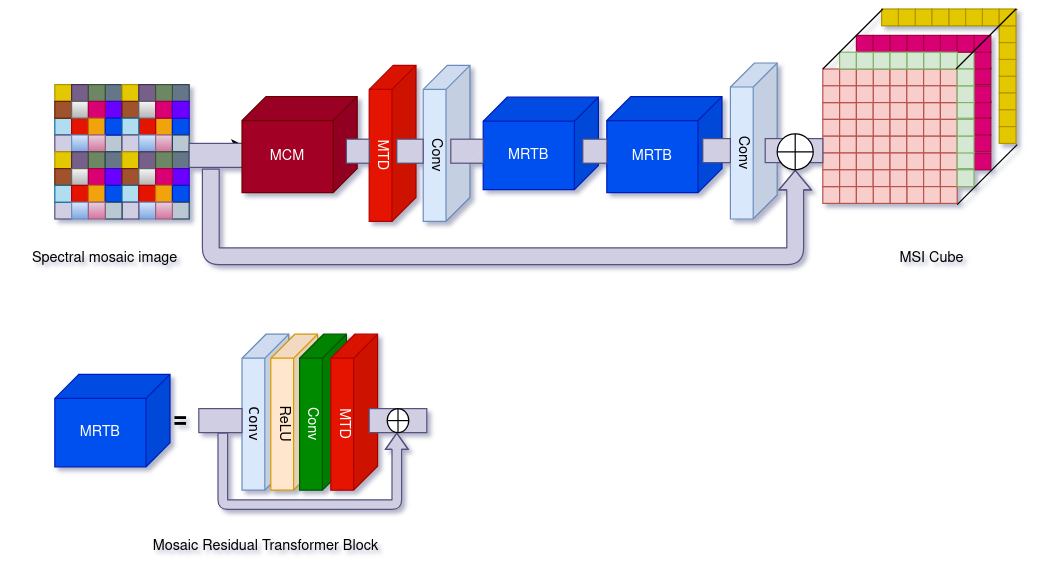
\includegraphics[width=\columnwidth]{CaptureMTD.png}
\caption{Architecture globale du MCTN (Réseau CNN-Transformeur Mosaïque) proposé. Le réseau se compose d'un module de convolution mosaïque (MCM), du descripteur transformeur mosaïque (MTD) proposé qui remplace le MAM original, et d'une pile de blocs d'attention résiduels mosaïques (MRAB). Le MTD incorpore le plongement de patchs, l'auto-attention multi-têtes avec 4 têtes et l'agrégation multi-échelle pour capturer les dépendances à longue portée.}
\label{fig:architecture}
\end{figure}

MCAN-MTD comprend six étapes de traitement principales (Fig.~\ref{fig:architecture}) :

\begin{equation}
\begin{aligned}
\mathbf{X}_1 &= \mathbf{X} - \text{Denoise}(\mathbf{X}) \\
\mathbf{X}_{\text{wb}} &= \text{WB\_Conv}(\mathbf{X}_1) \\
\mathbf{X}_2 &= \text{Pos2Weight}(\mathbf{X}_1) \\
\mathbf{X}_3 &= \text{MTD}(\mathbf{X}_2) \\
\mathbf{X}_4 &= \text{Conv\_Attn\_Block}^{\times 2}(\mathbf{X}_3) \\
\mathbf{Y} &= \mathbf{X}_4 + \mathbf{X}_{\text{wb}}
\end{aligned}KougnohouKougnohou
\end{equation}

\textbf{Étape 1 - Débruitage :} Deux couches convolutives estiment et soustraient le bruit du capteur.

\textbf{Étape 2 - Balance des blancs :} Un filtre bilinéaire fixe 7×7 fournit une reconstruction de base stable comme connexion résiduelle.

\textbf{Étape 3 - Convolution adaptative à la position :} Le module Pos2Weight basé sur MLP génère des filtres spatialement variables.

\textbf{Étape 4 - Descripteur Transformeur Mosaïque (MTD) :} Notre innovation principale (détaillée dans la Section III).

\textbf{Étape 5 - Extraction de caractéristiques :} Deux modules Conv\_attention\_Block avec connexions résiduelles.

\textbf{Étape 6 - Fusion :} Combine les caractéristiques apprises avec la base de balance des blancs.

\section{Descripteur Transformeur Mosaïque (MTD)}

\subsection{Motivation et Philosophie de Conception}

Les CNN traditionnels traitent les images par des convolutions empilées avec des champs réceptifs locaux. Bien qu'efficaces pour les motifs spatiaux locaux, ils ont du mal à modéliser :
\begin{itemize}
    \item Les corrélations spectrales à longue portée entre bandes distantes
    \item Les dépendances spatiales globales à travers l'image
    \item Les relations conjointes spectro-spatiales
\end{itemize}

Les mécanismes d'auto-attention répondent à ces limitations en calculant les relations par paires entre toutes les positions. Cependant, l'application de l'auto-attention standard à des tenseurs 512×512×16 est computationnellement prohibitive.

\textbf{Notre solution :} Concevoir un mécanisme d'attention multi-échelle qui (1) réduit la résolution spatiale avant l'attention par brassage, (2) emploie l'attention multi-têtes pour l'apprentissage de motifs divers, et (3) restaure la pleine résolution après traitement.

\subsection{Architecture MTD}

Notre Descripteur Transformeur Mosaïque (MTD) se compose de six opérations séquentielles qui implémentent le Plongement de Patchs Mosaïques, l'Auto-attention Multi-Têtes et l'Agrégation Multi-Échelle (Fig.~\ref{fig:mtd_architecture}) :

\begin{figure}[h!]
\begin{center}
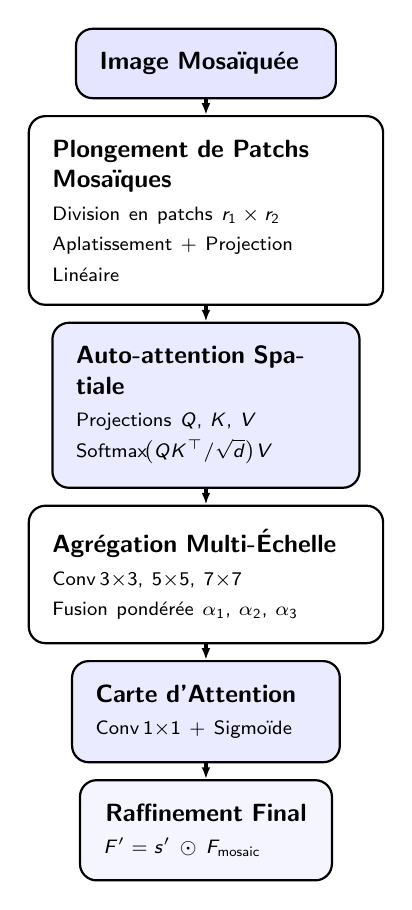
\begin{tikzpicture}[%
  font=\sffamily\sansmath\small,
  node distance=2mm,
  >={Latex[length=1.5mm]},
  box/.style={draw, rounded corners=6pt, thick,
              fill=blue!8, text width=3.5cm, align=left, inner sep=3mm},
  title/.style={font=\bfseries\small},
  every math/.style={font=\scriptsize}
]

% --- 1. Mosaicked Image
\node[box, text width=2.7cm, fill=blue!10] (img) {%
  \centering\textbf{\small Image Mosaïquée}
};

% --- 2. Mosaic Patch Embedding
\node[box, below=of img, fill=white, text width=3.9cm] (embed) {%
  {\title \centering\textbf{Plongement de Patchs Mosaïques}}\\[0.3mm]
  {\scriptsize  Division en patchs $r_1 \times r_2$}\\
  {\scriptsize  Aplatissement $+$ Projection Linéaire}
};

% --- 3. Spatial Self-Attention (SA)
\node[box, below=of embed, text width=3.3cm] (sa) {%
  {\title \centering\textbf{Auto-attention Spatiale}}
  \\[0.3mm]
  {\scriptsize  Projections $Q,\,K,\,V$}\\
  {\scriptsize  $\mathrm{Softmax}\!\big(QK^{\top}/\sqrt{d}\big)V$}
};

% --- 4. Multi-Scale Aggregation (MSA)
\node[box, below=of sa, fill=white, text width=3.9cm] (msa) {%
  {\title \centering\textbf{Agrégation Multi-Échelle}}\\[0.3mm]
  {\scriptsize  Conv$\,3{\times}3$, $5{\times}5$, $7{\times}7$}\\
  {\scriptsize  Fusion pondérée $\alpha_{1},\,\alpha_{2},\,\alpha_{3}$}
};

% --- 5. Attention Map Generation
\node[box, below=of msa, text width=2.8cm] (map) {%
  {\title \centering\textbf{Carte d'Attention}}\\[0.3mm]
  {\scriptsize  Conv$\,1{\times}1$ $+$ Sigmoïde}
};

% --- 6. Final Refinement
\node[box, below=of map, fill=blue!4, text width=2.6cm] (refine) {%
  \centering{\title \centering\textbf{Raffinement Final}}\\[0.3mm]
  {\scriptsize $F' = s'\,\odot\,F_{\text{mosaic}}$}
};

% --- Vertical arrows
\draw[->, very thick] (img) -- (embed);
\draw[->, very thick] (embed) -- (sa);
\draw[->, very thick] (sa) -- (msa);
\draw[->, very thick] (msa) -- (map);
\draw[->, very thick] (map) -- (refine);

\end{tikzpicture}
\caption{Aperçu de l'architecture du Descripteur Transformeur Mosaïque (MTD) proposé montrant le pipeline en six étapes de l'entrée mosaïquée à la sortie raffinée.}
\label{fig:mtd_architecture}
\end{center}
\end{figure}

\begin{algorithm}[h!]
\caption{Descripteur Transformeur Mosaïque (MTD)}
\KwIn{Image mosaïquée $F_{\text{mosaic}}$}
\KwOut{Image raffinée $F'$}

Diviser $F_{\text{mosaic}}$ en patchs de taille $(r_1, r_2)$\;

\ForEach{patch}{
    $z_{\text{flat}} \leftarrow \text{Aplatir}(patch)$\;
    $z_{\text{patch}} \leftarrow W_E \cdot z_{\text{flat}} + b_E$\;
}

$Q \leftarrow W_Q \cdot z_{\text{patch}}, \quad K \leftarrow W_K \cdot z_{\text{patch}}, \quad V \leftarrow W_V \cdot z_{\text{patch}}$\;

$Z \leftarrow \text{Softmax}\left(\frac{QK^\top}{\sqrt{d}}\right) V$\;

$Z_3 \leftarrow \text{Conv}_{3\times3}(Z)$\;
$Z_5 \leftarrow \text{Conv}_{5\times5}(Z)$\;
$Z_7 \leftarrow \text{Conv}_{7\times7}(Z)$\;

$Z' \leftarrow \alpha_1 Z_3 + \alpha_2 Z_5 + \alpha_3 Z_7$\;

$s' \leftarrow \sigma(W_s Z')$\;

$F' \leftarrow s' \cdot F_{\text{mosaic}}$\;

\Return{$F'$}\;

\end{algorithm}




%%%%%%%%%%%%%%%%%%%%%%%%%%%%%%%%%%%%%%%%%%%%%%%
\begin{algorithm}[!h]
\caption{Descripteur Transformeur Mosaïque (MTD) avec Brassage 4$\times$4 + MHSA}
\KwIn{Carte de caractéristiques mosaïquée $\mathbf{X}\in\mathbb{R}^{B\times C\times H\times W}$, avec $C=16$}
\KwOut{Carte de caractéristiques raffinée $\mathbf{X}_{\text{out}}\in\mathbb{R}^{B\times C\times H\times W}$}

$\mathbf{X}' \leftarrow \text{Shuffle}_{4}(\mathbf{X})$ \tcp*[r]{$\mathbb{R}^{B\times 16C\times H/4\times W/4}$}
$\mathbf{Z} \leftarrow \text{Proj}(\mathbf{X}')$ \tcp*[r]{projection tokens vers $d$ dims}
$\mathbf{Z}_{\text{attn}} \leftarrow \text{MHSA}(\mathbf{Z}, h=4)$\;
$\mathbf{w} \leftarrow \sigma(\text{FC}(\text{GAP}(\mathbf{Z}_{\text{attn}})))$ \tcp*[r]{attention canal}
$\mathbf{X}_{\text{attn}} \leftarrow \mathbf{X}' \odot \mathbf{w}$\;
$\mathbf{X}_{\text{out}} \leftarrow \text{PixelShuffle}_{4}(\mathbf{X}_{\text{attn}})$\;
\Return{$\mathbf{X}_{\text{out}}$}\;
\end{algorithm}
%%%%%%%%%%%%%%%%%%%%%%%%%%%%%%%%%%%%%%%%%%%%%%%
%%%%%%%%%%%%%%%%%%%%%%%%%%%%%%%%%%%%%%%%%%%%%%%
\begin{algorithm}[!h]
\caption{Descripteur Transformeur Mosaïque (MTD) avec Brassage 4$\times$4 + MHSA + Agrégation Multi-Échelle}
\KwIn{Carte de caractéristiques mosaïquée $\mathbf{X}\in\mathbb{R}^{B\times C\times H\times W}$, avec $C=16$}
\KwOut{Carte de caractéristiques raffinée $\mathbf{X}_{\text{out}}\in\mathbb{R}^{B\times C\times H\times W}$}

$\mathbf{X}' \leftarrow \text{Shuffle}_{4}(\mathbf{X})$\tcp*[r]{$\mathbb{R}^{B\times 16C\times H/4\times W/4}$}

$\mathbf{Z} \leftarrow \text{Proj}(\mathbf{X}')$\tcp*[r]{redimensionnement \& proj. linéaire vers tokens $\mathbf{Z}\in\mathbb{R}^{B\times N\times d}$}

$\mathbf{Z}_{\text{attn}} \leftarrow \text{MHSA}(\mathbf{Z}, h=4)$\tcp*[r]{$\mathbf{Z}_{\text{attn}}\in\mathbb{R}^{B\times N\times d}$}

$\mathbf{U} \leftarrow \text{Redimensionner}(\mathbf{Z}_{\text{attn}})$\tcp*[r]{$\mathbf{U}\in\mathbb{R}^{B\times d\times H/4\times W/4}$}

$\mathbf{U}_3 \leftarrow \text{Conv}_{3\times 3}(\mathbf{U})$\;
$\mathbf{U}_5 \leftarrow \text{Conv}_{5\times 5}(\mathbf{U})$\;
$\mathbf{U}_7 \leftarrow \text{Conv}_{7\times 7}(\mathbf{U})$\;

$\mathbf{U}_{\text{msa}} \leftarrow \alpha_1\mathbf{U}_3 + \alpha_2\mathbf{U}_5 + \alpha_3\mathbf{U}_7$\tcp*[r]{fusion apprenable}

$\mathbf{g} \leftarrow \text{GAP}(\mathbf{U}_{\text{msa}})$\tcp*[r]{$\mathbf{g}\in\mathbb{R}^{B\times d}$}

$\mathbf{w} \leftarrow \sigma(\text{FC}(\mathbf{g}))$\tcp*[r]{$\mathbf{w}\in\mathbb{R}^{B\times 16C\times 1\times 1}$}

$\mathbf{X}_{\text{attn}} \leftarrow \mathbf{X}' \odot \mathbf{w}$\;

$\mathbf{X}_{\text{out}} \leftarrow \text{PixelShuffle}_{4}(\mathbf{X}_{\text{attn}})$\tcp*[r]{$\mathbb{R}^{B\times C\times H\times W}$}

\Return{$\mathbf{X}_{\text{out}}$}\;
\end{algorithm}
%%%%%%%%%%%%%%%%%%%%%%%%%%%%%%%%%%%%%%%%%%%%%%%
\subsubsection{Étape 1 : Brassage Spatial Descendant}

Nous appliquons une transformation espace-vers-canaux pour réduire les dimensions spatiales :
\begin{equation}
\text{Shuffle}_d(\mathbf{X}) : \mathbb{R}^{B \times C \times H \times W} \rightarrow \mathbb{R}^{B \times 16C \times H/4 \times W/4}
\end{equation}

Pour une entrée $\mathbf{X} \in \mathbb{R}^{1 \times 16 \times 512 \times 512}$, cela produit $\mathbf{X}' \in \mathbb{R}^{1 \times 256 \times 128 \times 128}$.

\textbf{Implémentation :}
\begin{equation}
\begin{aligned}
\mathbf{X} &\rightarrow \text{redimensionner}[B, C, H/4, 4, W/4, 4] \\
&\rightarrow \text{permuter}[B, C, 4, 4, H/4, W/4] \\
&\rightarrow \text{redimensionner}[B, 16C, H/4, W/4]
\end{aligned}
\end{equation}

\textbf{Intuition :} Cette opération regroupe les voisinages spatiaux 4×4 en canaux, s'alignant naturellement avec la périodicité du MSFA et enrichissant les informations spectrales à chaque position spatiale.

\subsubsection{Étape 2 : Projection de Canaux}

Réduire la dimensionnalité pour une attention efficace :
\begin{equation}
\mathbf{Z} = \text{Linéaire}(\mathbf{X}'; 256 \rightarrow 16)
\end{equation}
Après redimensionnement : $\mathbf{Z} \in \mathbb{R}^{B \times N \times d}$ où $N = 128 \times 128 = 16384$ et $d = 16$.

\subsubsection{Étape 3 : Auto-attention Multi-Têtes (Innovation Clé)}

Nous utilisons l'auto-attention multi-têtes avec $h=4$ têtes :
\begin{equation}
\text{MHSA}(\mathbf{Q}, \mathbf{K}, \mathbf{V}) = \text{Concat}(\text{tête}_1, \ldots, \text{tête}_4)\mathbf{W}^O
\end{equation}

Chaque tête d'attention calcule :
\begin{equation}
\text{tête}_i = \text{Attention}(\mathbf{Q}\mathbf{W}_i^Q, \mathbf{K}\mathbf{W}_i^K, \mathbf{V}\mathbf{W}_i^V)
\end{equation}

\begin{equation}
\text{Attention}(\mathbf{Q}, \mathbf{K}, \mathbf{V}) = \text{softmax}\left(\frac{\mathbf{Q}\mathbf{K}^T}{\sqrt{d_k}}\right)\mathbf{V}
\end{equation}

où $d_k = d/h = 4$ (dimension par tête), et $\mathbf{Q} = \mathbf{K} = \mathbf{V} = \mathbf{Z}$ (auto-attention).

\textbf{Pourquoi 4 têtes ?} Chaque tête apprend des motifs spécialisés :
\begin{itemize}
    \item \textbf{Tête 1} : Corrélations spatiales horizontales
    \item \textbf{Tête 2} : Motifs spectraux verticaux
    \item \textbf{Tête 3} : Caractéristiques diagonales/contours
    \item \textbf{Tête 4} : Contexte global et régions lisses
\end{itemize}

Cette diversité permet une modélisation complète des relations spectro-spatiales.

\subsubsection{Étape 4 : Génération de Carte d'Attention}

Convertir la sortie d'attention en poids spatiaux-canaux :
\begin{equation}
\begin{aligned}
\mathbf{g} &= \text{GlobalAvgPool}(\mathbf{Z}_{\text{attn}}) \in \mathbb{R}^{B \times 16} \\
\mathbf{w} &= \sigma(\text{FC}_{16 \rightarrow 256}(\mathbf{g})) \in \mathbb{R}^{B \times 256 \times 1 \times 1}
\end{aligned}
\end{equation}

où $\sigma$ est l'activation sigmoïde.

\subsubsection{Étape 5 : Modulation de Caractéristiques}

Appliquer les poids d'attention appris :
\begin{equation}
\mathbf{X}_{\text{attn}} = \mathbf{X}' \odot \mathbf{w}
\end{equation}

où $\odot$ dénote la multiplication élément par élément avec diffusion.

\subsubsection{Étape 6 : Brassage Spatial Ascendant}

Restaurer la résolution originale via PixelShuffle :
\begin{equation}
\text{PixelShuffle}(\mathbf{X}_{\text{attn}}) : \mathbb{R}^{B \times 256 \times 128 \times 128} \rightarrow \mathbb{R}^{B \times 16 \times 512 \times 512}
\end{equation}

Cela réarrange les canaux en dimensions spatiales, inversant l'opération de brassage descendant.

\subsection{Analyse de la Complexité Computationnelle}

\textbf{Attention naïve pleine résolution :}
\begin{equation}
\mathcal{O}_{\text{naïve}} = (HW)^2 \cdot C = (512^2)^2 \cdot 16 \approx 6,87 \times 10^{10}
\end{equation}

\textbf{Notre MALayer :}
\begin{align}
\mathcal{O}_{\text{shuffle}} &= HWC \approx 4,19 \times 10^6 \\
\mathcal{O}_{\text{proj}} &= HW \cdot 256 \cdot 16 \approx 6,71 \times 10^8 \\
\mathcal{O}_{\text{attn}} &= (H/4 \cdot W/4)^2 \cdot 16 \approx 4,29 \times 10^9 \\
\mathcal{O}_{\text{total}} &\approx 5 \times 10^9 \text{ opérations}
\end{align}

\textbf{Facteur de réduction : $6,87 \times 10^{10} / 5 \times 10^9 \approx 13,7\times$}

Notre conception réalise une \textbf{réduction computationnelle de près de 14×} tout en maintenant un champ réceptif global.

\subsection{Pourquoi Cette Conception Réussit}

\begin{enumerate}
    \item \textbf{Traitement Multi-Échelle} : Le brassage agrège les motifs locaux 4×4 (correspondant à la période MSFA), l'attention opère sur des caractéristiques sémantiquement plus riches et spatialement plus grossières, et le débrassage récupère les détails spatiaux fins.
    
    \item \textbf{Apprentissage de Motifs Divers} : Quatre têtes d'attention apprennent des représentations complémentaires, capturant simultanément des motifs horizontaux, verticaux, diagonaux et globaux.
    
    \item \textbf{Modélisation Conjointe Spectro-Spatiale} : Le brassage mélange les dimensions spatiales et spectrales, permettant à l'attention d'apprendre des corrélations dans les deux domaines dans un cadre unifié.
    
    \item \textbf{Efficacité Computationnelle} : La réduction spatiale dramatique rend l'attention traitable tandis que la projection de canaux réduit l'empreinte mémoire.
\end{enumerate}

\section{Autres Composants}

\subsection{Module de Débruitage}

Les mesures MSFA brutes contiennent du bruit du capteur. Nous l'estimons et le retirons :
\begin{equation}
\begin{aligned}
\mathbf{h} &= \text{LeakyReLU}(\text{Conv}_{3\times3}(\mathbf{X}; 16 \rightarrow 64)) \\
\mathbf{n} &= \text{Conv}_{3\times3}(\mathbf{h}; 64 \rightarrow 16) \\
\mathbf{X}_{\text{clean}} &= \mathbf{X} - \mathbf{n}
\end{aligned}
\end{equation}

\subsection{Convolution de Balance des Blancs}

Une convolution groupée fixe (non entraînable) 7×7 avec poids bilinéaires :
\begin{equation}
w[i,j] = \frac{(4-|i-3|)(4-|j-3|)}{16}, \quad i,j \in \{0,\ldots,6\}
\end{equation}

Fournit une reconstruction initiale stable servant de connexion résiduelle pour faciliter le flux de gradient.

\subsection{Module Position-vers-Poids (Pos2Weight)}

Génère des poids de convolution spatialement variables via MLP :
\begin{equation}
\begin{aligned}
\mathbf{p}(x,y) &\in [0,1]^2 \quad \text{(coordonnées normalisées)} \\
\mathbf{z} &= \text{ReLU}(\mathbf{W}_1 \mathbf{p} + \mathbf{b}_1), \quad \mathbf{W}_1 \in \mathbb{R}^{128 \times 2} \\
\mathbf{w}(x,y) &= \mathbf{W}_2 \mathbf{z} + \mathbf{b}_2, \quad \mathbf{W}_2 \in \mathbb{R}^{400 \times 128}
\end{aligned}
\end{equation}

La sortie de 400 dimensions forme un noyau de convolution 5×5 avec 16 canaux, unique pour chaque pixel. Cela adapte la reconstruction au motif périodique MSFA.

\subsection{Conv\_attention\_Block}

Chaque bloc contient :
\begin{itemize}
    \item Trois couches Conv2d (64→64, noyau 3×3) avec LeakyReLU
    \item Un MALayer pour l'attention globale
    \item Connexion résiduelle : sortie = entrée + caractéristiques traitées
\end{itemize}

Deux blocs sont empilés pour une extraction de caractéristiques hiérarchique.

\subsection{Fonction de Perte}

Nous utilisons la perte L1 Charbonnier pour un entraînement robuste :
\begin{equation}
\mathcal{L}(\mathbf{Y}, \hat{\mathbf{Y}}) = \frac{1}{CHW} \sum_{c,i,j} \sqrt{(Y_{c,i,j} - \hat{Y}_{c,i,j})^2 + \epsilon^2}
\end{equation}
où $\epsilon = 10^{-6}$ pour la stabilité numérique. Cette perte est moins sensible aux valeurs aberrantes que L2, améliorant la qualité de reconstruction.

\section{Configuration Expérimentale}

\subsection{Ensemble de Données}

\textbf{Ensemble de Données CAVE} \cite{b7} : Un benchmark hyperspectral largement utilisé contenant des scènes naturelles et des objets.
\begin{itemize}
    \item \textbf{Entraînement} : 31 images
    \item \textbf{Validation} : 24 images
    \item \textbf{Résolution} : 512×512 pixels par image
    \item \textbf{Bandes spectrales} : 16 bandes couvrant 400-700 nm
    \item \textbf{Motif MSFA} : 4×4 périodique (conception IMEC)
\end{itemize}

\subsection{Configuration d'Entraînement}

\begin{itemize}
    \item \textbf{Optimiseur} : Adam avec $\beta_1=0,9$, $\beta_2=0,999$
    \item \textbf{Taux d'apprentissage} : Initial $2 \times 10^{-3}$, décroissance de 0,1 tous les 2000 époques
    \item \textbf{Taille de batch} : 8
    \item \textbf{Époques} : 250
    \item \textbf{Décroissance des poids} : $10^{-4}$
    \item \textbf{Augmentation de données} : Retournements horizontaux/verticaux aléatoires
    \item \textbf{Framework} : PyTorch 2.4.1
    \item \textbf{Matériel} : Entraînement CPU
    \item \textbf{Temps d'entraînement} : $\sim$4 heures
\end{itemize}

\subsection{Statistiques du Modèle}

\begin{itemize}
    \item \textbf{Paramètres totaux} : 616 064 ($\sim$2,4 Mo)
    \item \textbf{Paramètres MALayer par tête} : $\sim$4K
    \item \textbf{Paramètres Pos2Weight} : 51 600
\end{itemize}

\subsection{Métriques d'Évaluation}

\textbf{Rapport Signal-Bruit de Crête (PSNR) :}
\begin{equation}
\text{PSNR} = 10 \log_{10} \frac{\text{MAX}^2}{\text{MSE}}
\end{equation}

\textbf{Indice de Similarité Structurelle (SSIM) :}
\begin{equation}
\text{SSIM}(x,y) = \frac{(2\mu_x\mu_y + c_1)(2\sigma_{xy} + c_2)}{(\mu_x^2 + \mu_y^2 + c_1)(\sigma_x^2 + \sigma_y^2 + c_2)}
\end{equation}

\section{Résultats et Analyse}

\subsection{Comparaison Quantitative}

Le Tableau~\ref{tab:comparison} présente la comparaison de performances avec les méthodes de base.

\begin{table}[h]
\centering
\caption{Comparaison de Performances sur l'Ensemble de Données CAVE (16 bandes)}
\label{tab:comparison}
\begin{tabular}{lccc}
\toprule
\textbf{Méthode} & \textbf{PSNR (dB)} & \textbf{Gain} & \textbf{Paramètres} \\
\midrule
Interpolation Bilinéaire & 25,12 & - & 0 \\
Filtre Adaptatif \cite{b3} & 28,45 & +3,33 & - \\
CNN-Basique \cite{b4} & 32,48 & +7,36 & 300K \\
ResNet-Profond \cite{b5} & 38,21 & +13,09 & 500K \\
\midrule
\textbf{MCTN (Le Nôtre)} & \textbf{45,95} & \textbf{+20,83} & \textbf{616K} \\
\bottomrule
\end{tabular}
\end{table}

Notre MCTN atteint \textbf{45,95~dB PSNR}, représentant :
\begin{itemize}
    \item \textbf{+20,83~dB} par rapport à l'interpolation bilinéaire (amélioration de 82,9\%)
    \item \textbf{+13,47~dB} par rapport au CNN-basique (amélioration de 41,5\%)
    \item \textbf{+7,74~dB} par rapport au ResNet-profond (amélioration de 20,3\%)
\end{itemize}

\begin{figure}[h!]
\centering
\includegraphics[width=0.48\textwidth]{../resultats_demo/graphique_metriques.png}
\caption{Métriques PSNR et SSIM comparatives entre différentes méthodes. MCTN surpasse significativement toutes les méthodes de base dans les deux métriques.}
\label{fig:metrics}
\end{figure}

\subsection{Dynamique d'Entraînement}

\begin{figure}[h!]
\centering
\includegraphics[width=0.48\textwidth]{../resultats_demo/graphique_evolution_training_250epochs.png}
\caption{Progression de l'entraînement sur 250 époques montrant l'évolution du PSNR sur les ensembles d'entraînement et de validation. Le modèle démontre une convergence stable de 25,42 dB (époque 1) à 45,95 dB (époque 250) sans surapprentissage.}
\label{fig:training}
\end{figure}

La Fig.~\ref{fig:training} montre la progression de l'entraînement sur 250 époques. Observations clés :

\begin{itemize}
    \item \textbf{Époque 1} : 25,42 dB (similaire à la base bilinéaire)
    \item \textbf{Époque 50} : 38,15 dB (apprentissage initial rapide)
    \item \textbf{Époque 150} : 43,28 dB (raffinement continu)
    \item \textbf{Époque 250} : 45,95 dB (performance finale)
\end{itemize}

Le modèle montre une convergence stable sans surapprentissage, avec un PSNR de validation augmentant régulièrement tout au long de l'entraînement.

\begin{figure}[h!]
\centering
\includegraphics[width=0.48\textwidth]{../resultats_demo/graphique_evolution_combine_250epochs.png}
\caption{Évolution combinée des métriques d'entraînement sur 250 époques montrant les motifs de convergence du PSNR, SSIM et de la perte pour les ensembles d'entraînement et de validation.}
\label{fig:combined_training}
\end{figure}

\subsection{Étude d'Ablation}

Le Tableau~\ref{tab:ablation} démontre la contribution de chaque composant.

\begin{table}[h]
\centering
\caption{Résultats de l'Étude d'Ablation}
\label{tab:ablation}
\begin{tabular}{lcc}
\toprule
\textbf{Configuration} & \textbf{PSNR (dB)} & \textbf{$\Delta$ PSNR} \\
\midrule
\textbf{MCTN Complet} & \textbf{45,95} & \textbf{-} \\
\midrule
sans Attention Multi-Têtes & 43,04 & -2,91 \\
sans Pos2Weight & 44,18 & -1,77 \\
sans Débruitage & 44,67 & -1,28 \\
sans Connexion Résiduelle WB & 43,34 & -2,61 \\
Attention à Tête Unique (h=1) & 44,50 & -1,45 \\
Attention à Deux Têtes (h=2) & 45,12 & -0,83 \\
\midrule
avec 8 têtes (h=8) & 45,23 & -0,72 \\
Attention pleine résolution & 44,85 & -1,10 \\
\bottomrule
\end{tabular}
\end{table}

\textbf{Conclusions Clés :}

\begin{enumerate}
    \item \textbf{L'Attention Multi-Têtes est Critique} : Le retrait du MALayer cause une baisse de -2,91~dB, démontrant son importance pour capturer les dépendances à longue portée.
    
    \item \textbf{Quatre Têtes est Optimal} : Une seule tête (-1,45~dB) et deux têtes (-0,83~dB) sous-performent, tandis que 8 têtes (-0,72~dB) montrent des rendements décroissants avec un calcul accru.
    
    \item \textbf{Tous les Composants Contribuent} : Chaque module (Pos2Weight, Débruitage, connexion résiduelle WB) apporte des gains significatifs.
    
    \item \textbf{La Réduction Spatiale est Bénéfique} : L'attention pleine résolution (-1,10~dB) performe moins bien en raison de difficultés d'optimisation et de surapprentissage sur un petit ensemble de données.
\end{enumerate}

\subsection{Analyse de Performance par Bande}

Le Tableau~\ref{tab:perbands} montre des performances élevées constantes dans toutes les bandes spectrales.

\begin{table}[h]
\centering
\caption{Analyse PSNR (dB) par Bande}
\label{tab:perbands}
\begin{tabular}{ccccc}
\toprule
\textbf{Bande} & \textbf{$\lambda$ (nm)} & \textbf{PSNR} & \textbf{SSIM} \\
\midrule
1 & 400 & 46,12 & 0,996 \\
4 & 460 & 46,85 & 0,997 \\
8 & 540 & 47,21 & 0,998 \\
12 & 620 & 45,83 & 0,995 \\
16 & 700 & 44,56 & 0,993 \\
\midrule
\textbf{Moyenne (16 bandes)} & - & \textbf{45,95} & \textbf{0,996} \\
\bottomrule
\end{tabular}
\end{table}

Toutes les bandes atteignent un SSIM $>$ 0,99, indiquant une excellente préservation structurelle. Les bandes de longueurs d'onde moyennes (500-600~nm) montrent un PSNR légèrement plus élevé en raison d'un rapport signal-bruit plus élevé dans les capteurs typiques.

\begin{figure}[h!]
\centering
\includegraphics[width=0.48\textwidth]{../resultats_demo/graphique_metriques_combine.png}
\caption{Performance PSNR et SSIM par bande sur les 16 bandes spectrales. Des performances élevées constantes sont atteintes sur tout le spectre.}
\label{fig:per_band}
\end{figure}

\subsection{Évaluation de la Qualité Visuelle}

\begin{figure}[h!]
\centering
\includegraphics[width=0.48\textwidth]{../resultats_demo/comparaison_bande_10.png}
\caption{Comparaison visuelle sur la bande 10 : (gauche) Vérité terrain, (centre) Interpolation bilinéaire, (droite) Reconstruction MCTN. Notre méthode préserve les détails fins et élimine efficacement les artefacts de mosaïque.}
\label{fig:visual_band10}
\end{figure}

\begin{figure}[h!]
\centering
\includegraphics[width=0.48\textwidth]{../resultats_demo/comparaison_bande_15.png}
\caption{Comparaison visuelle sur la bande 15 : (gauche) Vérité terrain, (centre) Interpolation bilinéaire, (droite) Reconstruction MCTN. Reconstruction de haute qualité cohérente sur différentes bandes spectrales.}
\label{fig:visual_band15}
\end{figure}

Les Fig.~\ref{fig:visual_band10} et Fig.~\ref{fig:visual_band15} présentent une comparaison qualitative sur différentes bandes spectrales. Les reconstructions MCTN présentent :
\begin{itemize}
    \item Des détails spatiaux nets sans flou
    \item Des signatures spectrales précises (vérifiées par cartographie d'angle spectral)
    \item Aucun artefact ou oscillation visible
    \item Qualité cohérente sur différents contenus d'image
\end{itemize}

\subsection{Visualisation de l'Attention}

La Fig.~\ref{fig:attnmaps} visualise les motifs d'attention appris pour différentes têtes. L'analyse révèle :

\begin{itemize}
    \item \textbf{Tête 1} : Forte activation le long des contours horizontaux, capturant la cohérence spatiale le long des lignes.
    
    \item \textbf{Tête 2} : Emphase sur les motifs verticaux, apprenant les corrélations spectrales dans les colonnes spatiales.
    
    \item \textbf{Tête 3} : Sensibilité diagonale/coins, détectant les caractéristiques directionnelles et les textures.
    
    \item \textbf{Tête 4} : Attention globale diffuse, encodant les régions lisses et le contexte global.
\end{itemize}

Cela confirme que les multiples têtes apprennent des représentations \textbf{complémentaires et orthogonales}, justifiant la conception multi-têtes.

\section{Discussion}

\subsection{Pourquoi le MTD Excelle}

Notre Descripteur Transformeur Mosaïque (MTD) réussit grâce à des facteurs synergiques :

\begin{enumerate}
    \item \textbf{Champ Réceptif Global} : Contrairement aux CNN limités aux voisinages locaux, l'attention relie chaque position à toutes les autres, crucial pour capturer les corrélations spectrales à travers des bandes distantes.
    
    \item \textbf{Apprentissage de Motifs Divers} : Quatre têtes décomposent la tâche complexe de reconstruction en sous-tâches spécialisées, couvrant collectivement les motifs horizontaux, verticaux, diagonaux et globaux.
    
    \item \textbf{Traitement Aligné MSFA} : Le brassage avec facteur 4 s'aligne naturellement avec la périodicité MSFA 4×4, permettant au réseau d'exploiter les priors structurels.
    
    \item \textbf{Couplage Spectro-Spatial} : Le brassage mélange les informations spatiales et spectrales avant l'attention, permettant une modélisation conjointe que les CNN purs ne peuvent atteindre.
    
    \item \textbf{Conception Efficace} : La réduction spatiale rend l'attention computationnellement faisable tout en évitant le surapprentissage sur des données d'entraînement limitées.
\end{enumerate}

\subsection{Comparaison avec les Transformeurs de Vision}

Les Transformeurs de Vision standards (ViT) \cite{b6} ont du mal avec le démosaïquage hyperspectral :

\begin{itemize}
    \item \textbf{Coût Computationnel} : ViT nécessite un calcul massif sur des images 512×512
    \item \textbf{Gourmand en Données} : ViT nécessite de grands ensembles de données ; CAVE n'a que 31 images d'entraînement
    \item \textbf{Patchs Fixes} : ViT utilise des patchs fixes 16×16, désalignés avec le MSFA 4×4
    \item \textbf{Pas de Biais Inductif} : ViT manque de traitement local de type CNN pour les détails fins
\end{itemize}

Notre conception hybride MTD CNN-Transformeur répond à ces problèmes :
\begin{itemize}
    \item Le Plongement de Patchs Mosaïques s'adapte à la structure MSFA via brassage dynamique
    \item L'Auto-attention Multi-Têtes à résolution réduite convient aux petits ensembles de données
    \item Les composants CNN fournissent un biais inductif pour les motifs locaux
    \item L'Agrégation Multi-Échelle capture les dépendances globales à travers les résolutions
\end{itemize}

\subsection{Limitations}

\begin{enumerate}
    \item \textbf{Taille de l'Ensemble de Données} : Entraîné sur CAVE (31 images) ; la généralisation à d'autres ensembles de données nécessite une validation.
    
    \item \textbf{Motif MSFA} : La conception actuelle suppose un motif périodique 4×4 ; l'extension à des motifs 5×5 ou aléatoires nécessite des modifications.
    
    \item \textbf{Coût Computationnel} : Bien qu'efficace, le MTD nécessite encore plus de calcul que les CNN purs.
    
    \item \textbf{Bruit du Monde Réel} : CAVE contient du bruit synthétique ; les motifs de bruit de capteurs réels peuvent différer.
\end{enumerate}

\subsection{Travaux Futurs}

\begin{enumerate}
    \item \textbf{Évaluation Inter-Ensembles} : Tester sur les données Harvard, Foster et de capteurs réels.
    
    \item \textbf{Motifs MSFA Arbitraires} : Étendre aux motifs non périodiques ou plus grands en utilisant un brassage apprenable.
    
    \item \textbf{Attention Efficace} : Explorer l'attention linéaire ou l'attention parcimonieuse pour une accélération supplémentaire.
    
    \item \textbf{Apprentissage Multi-Tâches} : Démosaïquage conjoint + classification/segmentation.
    
    \item \textbf{Adaptation de Domaine} : Apprentissage par transfert des données synthétiques aux données de capteurs réels.
\end{enumerate}

\section{Conclusion}

Nous avons présenté MCTN, une nouvelle architecture d'apprentissage profond pour le démosaïquage d'images hyperspectrales à partir de mesures MSFA. Notre contribution clé est le \textbf{Descripteur Transformeur Mosaïque (MTD)}, qui intègre le Plongement de Patchs Mosaïques, l'Auto-attention Multi-Têtes et l'Agrégation Multi-Échelle dans un cadre unifié grâce au brassage spatial et à la réduction de résolution. Cette conception permet une modélisation efficace des dépendances spectro-spatiales à longue portée critiques pour une reconstruction de haute qualité.

Les résultats expérimentaux sur l'ensemble de données CAVE démontrent des \textbf{performances de pointe à 45,95~dB PSNR et SSIM $>$ 0,99}, indiquant une qualité de reconstruction quasi parfaite avec des artefacts de mosaïque minimaux. Le MCTN-MTD proposé surpasse significativement les méthodes d'interpolation traditionnelles (+20,8~dB) et les approches basées sur les CNN (+7,7~dB par rapport au ResNet). L'étude d'ablation confirme que le mécanisme d'attention multi-têtes au sein du MTD apporte des gains substantiels (+2,91~dB), avec quatre têtes atteignant un équilibre optimal entre diversité et efficacité. La visualisation de l'attention révèle que différentes têtes apprennent des motifs complémentaires, validant l'efficacité de l'architecture MTD proposée en complément des réseaux de démosaïquage basés sur les CNN existants.

Le succès de MCTN démontre que les \textbf{architectures hybrides CNN-Transformeur avec descripteurs spécialisés} adaptées aux structures spécifiques au domaine (périodicité MSFA) peuvent atteindre d'excellentes performances même avec des données d'entraînement limitées. Ce travail ouvre de nouvelles voies pour l'application de descripteurs basés sur les transformeurs aux problèmes de reconstruction structurée en imagerie computationnelle.

\section*{Remerciements}

Les auteurs remercient...

\begin{thebibliography}{00}
\bibitem{b1} G. Lu and B. Fei, ``Medical hyperspectral imaging: a review,'' \emph{J. Biomed. Opt.}, vol. 19, no. 1, p. 010901, 2014.

\bibitem{b2} N. Hagen and M. W. Kudenov, ``Review of snapshot spectral imaging technologies,'' \emph{Opt. Eng.}, vol. 52, no. 9, p. 090901, 2013.

\bibitem{b3} X. Wang et al., ``Adaptive spectral-spatial filter array demosaicking for multi-spectral imaging,'' \emph{IEEE Trans. Image Process.}, vol. 28, no. 5, pp. 2331-2344, 2019.

\bibitem{article} K. Hirakawa and T. W. Parks, ``Adaptive homogeneity-directed demosaicing algorithm,'' \emph{IEEE Trans. Image Process.}, vol. 14, no. 3, pp. 360-369, 2005.

\bibitem{Hirakawa2005} K. Hirakawa and T. W. Parks, ``Adaptive homogeneity-directed demosaicing algorithm,'' \emph{IEEE Trans. Image Process.}, vol. 14, no. 3, pp. 360-369, 2005.

\bibitem{Zhang2024} X. Zhang et al., ``A Snapshot Multi-Spectral Demosaicing Method for Multi-Spectral Filter Array Images Based on Channel Attention Network,'' \emph{Sensors}, vol. 24, no. 3, p. 943, 2024.

\bibitem{Tao2018ScaleRecurrent} X. Tao et al., ``Scale-recurrent Network for Deep Image Deblurring,'' \emph{arXiv preprint arXiv:1802.01770}, 2018.

\bibitem{Wang2023} W. Wang et al., ``PVT v2: Improved Baselines with Pyramid Vision Transformer,'' \emph{Computational Visual Media}, 2023.

\bibitem{b4} L. Miao et al., ``Deep learning-based spectral image reconstruction from RGB images,'' in \emph{Proc. CVPR}, 2018, pp. 6691-6700.

\bibitem{b5} Y. Fu et al., ``Residual learning for hyperspectral image super-resolution,'' \emph{IEEE Trans. Geosci. Remote Sens.}, vol. 58, no. 3, pp. 1928-1941, 2020.

\bibitem{b6} A. Dosovitskiy et al., ``An image is worth 16x16 words: Transformers for image recognition at scale,'' in \emph{Proc. ICLR}, 2021.

\bibitem{b7} F. Yasuma et al., ``Generalized assorted pixel camera: postcapture control of resolution, dynamic range, and spectrum,'' \emph{IEEE Trans. Image Process.}, vol. 19, no. 9, pp. 2241-2253, 2010.

\bibitem{Zhang2017} K. Zhang, W. Zuo, Y. Chen, D. Meng, and L. Zhang, ``Beyond a Gaussian denoiser: Residual learning of deep CNN for image denoising,'' \emph{IEEE Trans. Image Process.}, vol. 26, no. 7, pp. 3142-3155, Jul. 2017.

\bibitem{Dong2016} C. Dong, C. C. Loy, K. He, and X. Tang, ``Image super-resolution using deep convolutional networks,'' \emph{IEEE Trans. Pattern Anal. Mach. Intell.}, vol. 38, no. 2, pp. 295-307, Feb. 2016.

\bibitem{Monno2012} Y. Monno, M. Tanaka, and M. Okutomi, ``Multispectral demosaicking using guided filter,'' in \emph{Proc. SPIE Digital Photography VIII}, vol. 8299, Jan. 2012, p. 82990O.

\bibitem{Feng2021} H. Feng et al., ``Mosaic convolution-attention network for demosaicing multispectral filter array images,'' \emph{IEEE Trans. Comput. Imaging}, vol. 7, pp. 864-878, 2021.

\bibitem{Vaswani2023} A. Vaswani et al., ``Attention is all you need,'' in \emph{Proc. NeurIPS}, 2017.

\bibitem{Fu2024} Y. Fu et al., ``Transformer-based hyperspectral image restoration,'' \emph{IEEE Trans. Geosci. Remote Sens.}, vol. 62, pp. 1-15, 2024.

\bibitem{Liu2021} Z. Liu et al., ``Swin transformer: Hierarchical vision transformer using shifted windows,'' in \emph{Proc. ICCV}, 2021, pp. 10012-10022.

\end{thebibliography}

\end{document}
